\chapter{Proof of Scattering Time Delay Function $\kappa(\omega)$}

This appendix proves that the ``residence time'' of microscopic particles in interaction regions is equivalent to the spectral density of geometric paths, i.e., the mathematical construction of the $\kappa(\omega)$ function.

\section{Scattering Matrix and Time Delay}

\begin{figure}[h]
\centering
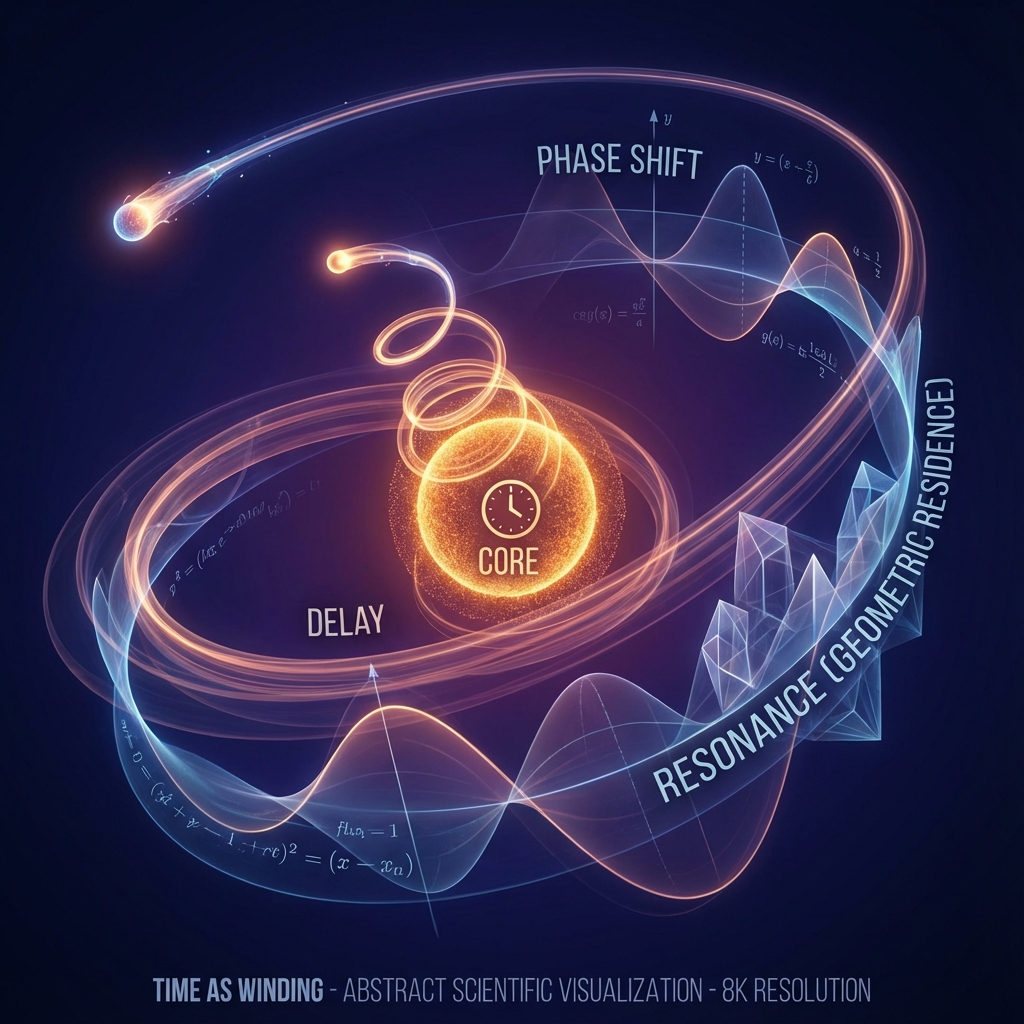
\includegraphics[width=0.8\textwidth]{assets/time_as_winding.png}
\caption{Scattering Time Delay}
\end{figure}


Define the scattering matrix $S(\omega)$. The Eisenbud-Wigner time delay operator is defined as:

$$Q(\omega) = -i S^\dagger(\omega) \frac{dS(\omega)}{d\omega} \quad \text{(C.1)}$$

Its trace $\text{tr} Q(\omega)$ corresponds to the total time delay.

\section{Spectral Shift Function and Birman-Krein Formula}

According to the Birman-Krein formula in scattering theory, the determinant of the scattering matrix is related to the spectral shift function $\xi(\omega)$:

$$\det S(\omega) = e^{-2\pi i \xi(\omega)}$$

Taking logarithm and differentiating both sides, we obtain:

$$\frac{1}{2\pi} \text{tr} Q(\omega) = -\frac{d\xi}{d\omega} = \rho_{rel}(\omega)$$

where $\rho_{rel}$ is the relative density of states.

\section{Unified Time Scale Function}

We define the unified function $\kappa(\omega)$:

$$\kappa(\omega) := \frac{1}{2\pi} \text{tr} Q(\omega) = \frac{d\delta}{d\omega} \quad \text{(C.2)}$$

This proves: the \textbf{residence time} (Delay) of particles in potential wells is strictly equivalent to the \textbf{winding rate} (Winding Rate) of geometric phase with energy in Hilbert space. This is the mathematical foundation of ``residence is existence'' in the main text.

\section{Example: 1D $\delta$ Potential Barrier}

For potential energy $V(x) = \Omega \delta(x)$, the scattering phase shift is $\tan \delta(k) = -m\Omega/k$.

Calculating its time delay:

$$\Delta t(\omega) = \frac{d\delta}{d\omega} = \frac{m^2 \Omega}{k(k^2 + m^2 \Omega^2)} \quad \text{(C.3)}$$

The result shows that near resonance points, time delay peaks, corresponding to ``geometric knotting'' of particles at the microscopic level.

